
\ifdefined\ishandout
\documentclass[11pt,english,handout]{beamer}
\else
\documentclass[11pt,english]{beamer}
\fi

%\documentclass[11pt]{beamer}
\usepackage{mathptmx}
\renewcommand{\sfdefault}{lmss}
\renewcommand{\familydefault}{\sfdefault}
\usepackage[T1]{fontenc}
\usepackage[latin9]{inputenc}
\usepackage{amsmath}
\usepackage{amssymb}
\usepackage{graphicx}
\PassOptionsToPackage{normalem}{ulem}
\usepackage{ulem}
\usepackage{caption}
\captionsetup{labelformat=empty}
\usepackage{bbm}
\usepackage{upgreek}
\usepackage{graphicx}
\setbeamertemplate{section in toc}[sections numbered]
\makeatletter
\usepackage{caption} 
\usepackage{bm}
\usepackage{subfig}
\captionsetup[table]{skip=10pt}
\usepackage{pdflscape}
%%%%%%%%%%%%%%%%%%%%%%%%%%%%%% Textclass specific LaTeX commands.
% this default might be overridden by plain title style
\newcommand\makebeamertitle{\frame{\maketitle}}%
% (ERT) argument for the TOC
\AtBeginDocument{%
	\let\origtableofcontents=\tableofcontents
	\def\tableofcontents{\@ifnextchar[{\origtableofcontents}{\gobbletableofcontents}}
	\def\gobbletableofcontents#1{\origtableofcontents}
}

%%%%%%%%%%%%%%%%%%%%%%%%%%%%%% User specified LaTeX commands.
%\documentclass[presentation]{beamer}


\def\Tiny{\fontsize{7pt}{8pt}\selectfont}
\def\Normal{\fontsize{8pt}{10pt}\selectfont}

\usetheme{Madrid}
\usecolortheme{lily}
%\setbeamercovered{transparent}
\useinnertheme{rounded}


\setbeamertemplate{footline}{\hfill\Normal{\insertframenumber/\inserttotalframenumber}}
%\setbeamertemplate{footline}{}

\setbeamertemplate{navigation symbols}{}

\newenvironment{changemargin}[2]{%
	\begin{list}{}{%
			\setlength{\topsep}{0pt}%
			\setlength{\leftmargin}{#1}%
			\setlength{\rightmargin}{#2}%
			\setlength{\listparindent}{\parindent}%
			\setlength{\itemindent}{\parindent}%
			\setlength{\parsep}{\parskip}% 
		}%
		\item[]}{\end{list}}

\setbeamertemplate{footline}{\hfill\insertframenumber/\inserttotalframenumber}
\setbeamertemplate{navigation symbols}{}

%\usepackage{times}  % fonts are up to you
\usepackage{graphicx}
%\usepackage{graphics}
\usepackage{epsfig}
\usepackage{bm}
\usepackage{epsf}
\usepackage{float}
\usepackage[final]{pdfpages}
\usepackage{multirow}
\usepackage{colortbl}
\usepackage{xkeyval}
%\usepackage{sgame}
%\usepackage{pst-node}
\usepackage{listings}
\usepackage{ifthen}
%\usepackage{hyperref}
\usepackage{tikz}

%\usepackage{times}  % fonts are up to you
%\usepackage{graphicx}
%\usepackage{graphics}
\usepackage{epsfig,bm,epsf,float}
\usepackage[final]{pdfpages}
\usepackage{xcolor,multirow,colortbl}
\usepackage{xkeyval}
\usepackage{verbatim}
%\usepackage{sgame}
%\usepackage{pst-node}
\usepackage{listings}
%\usepackage{handoutWithNotes}
%\pgfpagesuselayout{3 on 1 with notes}[letterpaper,border shrink=5mm]
%\pgfpagesuselayout{2 on 1 with notes landscape}[letterpaper,border shrink=5mm]
\usepackage{setspace}
\usepackage{ragged2e}
\usepackage{pdfpages}
\setbeamersize{text margin left=1em,text margin right=1em} % CambridgeUS spacing if you use default instead


%\pdfmapfile{+sansmathaccent.map}

% Table formatting
\usepackage{booktabs}


% Decimal align
\usepackage{dcolumn}
\newcolumntype{d}[0]{D{.}{.}{5}}


\global\long\def\expec#1{\mathbb{E}\left[#1\right]}
\global\long\def\var#1{\mathrm{Var}\left[#1\right]}
\global\long\def\cov#1{\mathrm{Cov}\left[#1\right]}
\global\long\def\prob#1{\mathrm{Prob}\left[#1\right]}
\global\long\def\one{\mathbf{1}}
\global\long\def\diag{\operatorname{diag}}
\global\long\def\expe#1#2{\mathbb{E}_{#1}\left[#2\right]}
\DeclareMathOperator*{\plim}{\text{plim}}

%\usefonttheme[onlymath]{serif}

\usepackage{appendixnumberbeamer}
\renewcommand{\thefootnote}{}

\setbeamertemplate{footline}
{
	\leavevmode%
	%   \hbox{%
	%      \begin{beamercolorbox}[wd=\paperwidth,ht=2.25ex,dp=1ex,right]{date in head/foot}%
	%\usebeamerfont{date in head/foot}\insertshortdate{}\hspace*{2em}%
	\hfill
	%turning the next line into a comment, erases the frame numbers
	\insertframenumber{}\hspace*{2ex}\vspace{1ex}
	
	%    \end{beamercolorbox}}%
}

\definecolor{blue}{RGB}{0, 0, 210}
\definecolor{red}{RGB}{170, 0, 0}

\makeatother

\usepackage[english]{babel}

\usepackage{tikz}
\newcommand*\circled[1]{\tikz[baseline=(char.base)]{             \node[circle,ball color=structure.fg, shade,   color=white,inner sep=1.2pt] (char) {\tiny #1};}} 

\makeatletter
\let\save@measuring@true\measuring@true
\def\measuring@true{%
	\save@measuring@true
	\def\beamer@sortzero##1{\beamer@ifnextcharospec{\beamer@sortzeroread{##1}}{}}%
	\def\beamer@sortzeroread##1<##2>{}%
	\def\beamer@finalnospec{}%
}
\makeatother



\setbeamersize{text margin left= .8em,text margin right=1em} 
\newenvironment{wideitemize}{\itemize\addtolength{\itemsep}{10pt}}{\enditemize}
\newenvironment{wideitemizeshort}{\itemize}{\enditemize}

\newcommand{\indep}{\perp\!\!\!\!\perp} 


\DeclareMathOperator*{\argmax}{arg\,max}
\DeclareMathOperator*{\argmin}{arg\,min}

\begin{document}
	
	%% Title slide
	\begin{frame}[noframenumbering]{}
		\vspace{0.5cm}
		\title[]{Chapter 8: Regression Discontinuity}
		\author{Jonathan Roth}
		\date{Mathematical Econometrics I \\ Brown University\\Fall 2023} 
		\titlepage {\small{}\ }\thispagestyle{empty} \vspace{-30pt}
		
	\end{frame}

	
	\begin{frame}{Motivation}
		
		\vspace{0.2cm}
		\begin{wideitemize}
			\item
			The key challenge in causal inference is finding a control group that is comparable to treated units in all ways except for treatment status\pause{}
			
			\item
			We've seen so far how to estimate causal effects when:\smallskip\pause{}
			\begin{itemize}
			\item The treatment is literally randomly assigned \smallskip\pause{}
			\item The treatment is as-good-as-randomly assigned\smallskip\pause{}
			\item Selection bias is constant over time (parallel trends)\smallskip\pause{}
			\item We have an as-good-as-random and excludable instrument
			\end{itemize} 
						
			\pause
			\item
			Today we will see another strategy: \textbf{regression discontinuity (RD)}
			
			\pause			
			\item
			The idea behind RD is that sometimes treatment status is (partially) determined by whether a score is above/below a threshold
			\pause\smallskip
				\begin{itemize}
					\item 
					For example, whether you are admitted to a school or university may depend on whether your test score exceeds a certain cutoff score
				\end{itemize} 
			
			\pause
			\item
			In such cases, RD compares outcomes for people with scores just above the threshold to people with scores just below the threshold
		\end{wideitemize}
		
	\end{frame}


	\begin{frame}{Example - Hou and Chao (2008)}
		\begin{wideitemize}
			\item
			Hu and Chao (2008) are interested in the question: does lack of health insurance prevent poor people from getting important medical care? 
			
			\pause
			\item
			Why don't they just compare medical care utilization between people with and without health insurance?
			\pause
				\begin{itemize}
					\item 
					Confounding variables! People with health insurance may be richer, which also may affect health directly
				\end{itemize}
			
			\pause
			\item
			Context: the Republic of Georgia (not the state!) created a health insurance program in 2006. Each household received a ``poverty score'' derived from 80 household variables, and households with a score $\leq$100,000 received health insurance
			
			\pause
			\item
			Key idea: people with scores just above 100,000 may be very similar to people with scores just below 100,000\smallskip\pause{}
			\begin{itemize}
			\item Except those below 100,000 had the health insurance treatment!
			\end{itemize}
		\end{wideitemize}
	\end{frame}
	
	\begin{frame}
		\centering
		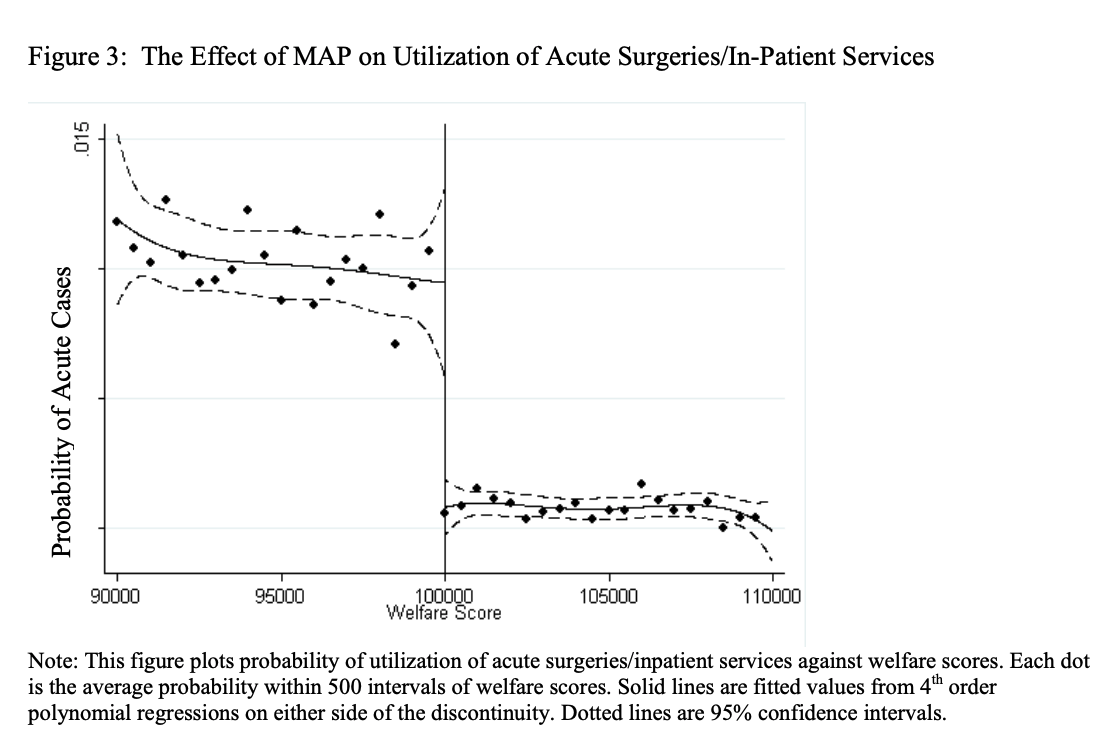
\includegraphics[width = 0.7\linewidth]{hou-rdd-basic}
		\begin{wideitemize}
			\item
			This plot shows outcomes (acute surgeries) as a function of the score
		\end{wideitemize}	
	\end{frame}

	\begin{frame}
	\centering
	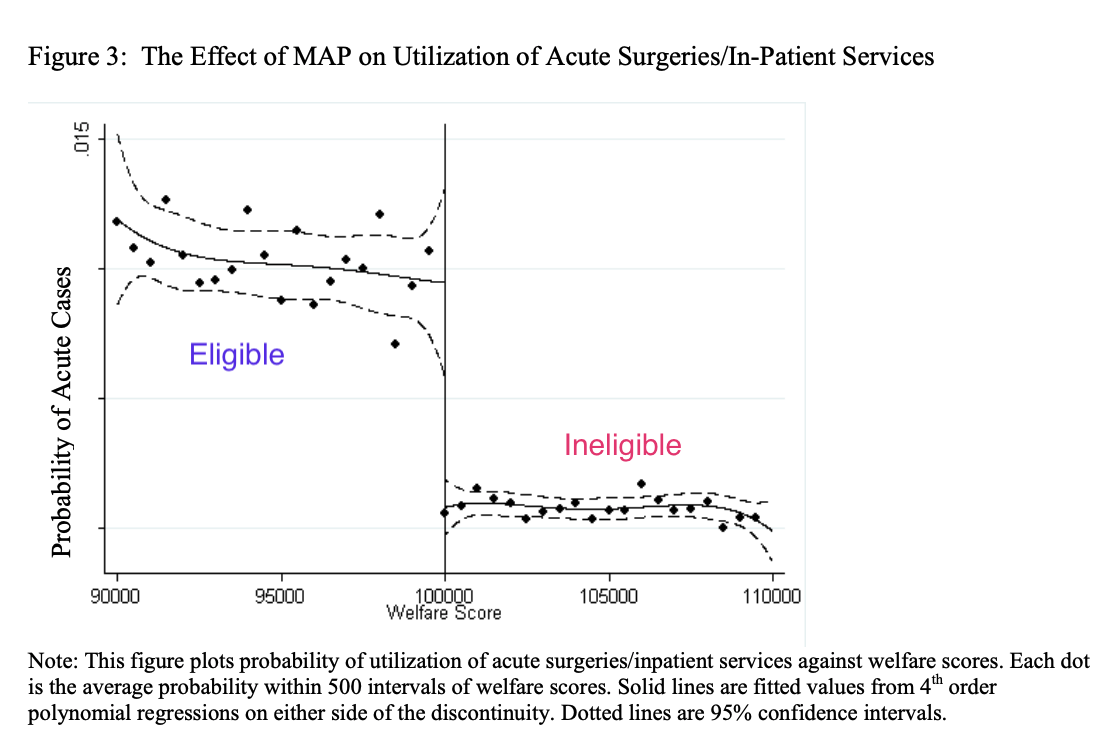
\includegraphics[width = 0.7\linewidth]{hou-rdd-eligibility}
	\begin{wideitemize}
		\item
		People to the left of the vertical line (at 100,000) receive health insurance from the government
		
		\item
		We might expect people with scores just below 100,000 to be very similar to people just above 100,000 on all factors other than healthcare eligibility
	\end{wideitemize}	
\end{frame}

	\begin{frame}
	\centering
	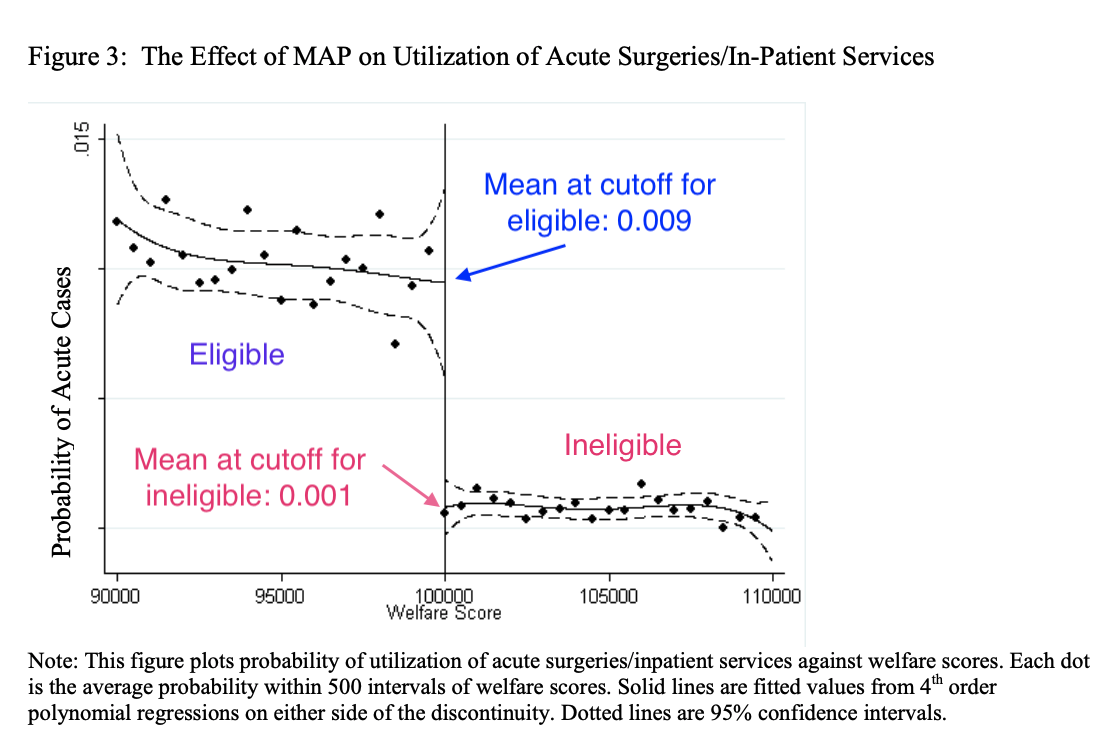
\includegraphics[width = 0.7\linewidth]{hou-rdd-means}
	\begin{wideitemize}
		\item
		We might expect people with scores just below 100,000 to be very similar to people just above 100,000 on all factors other than healthcare eligibility
		
		\item
		But people just below the threshold seem to get a lot more surgeries!
	\end{wideitemize}	
\end{frame}

	\begin{frame}
	\centering
	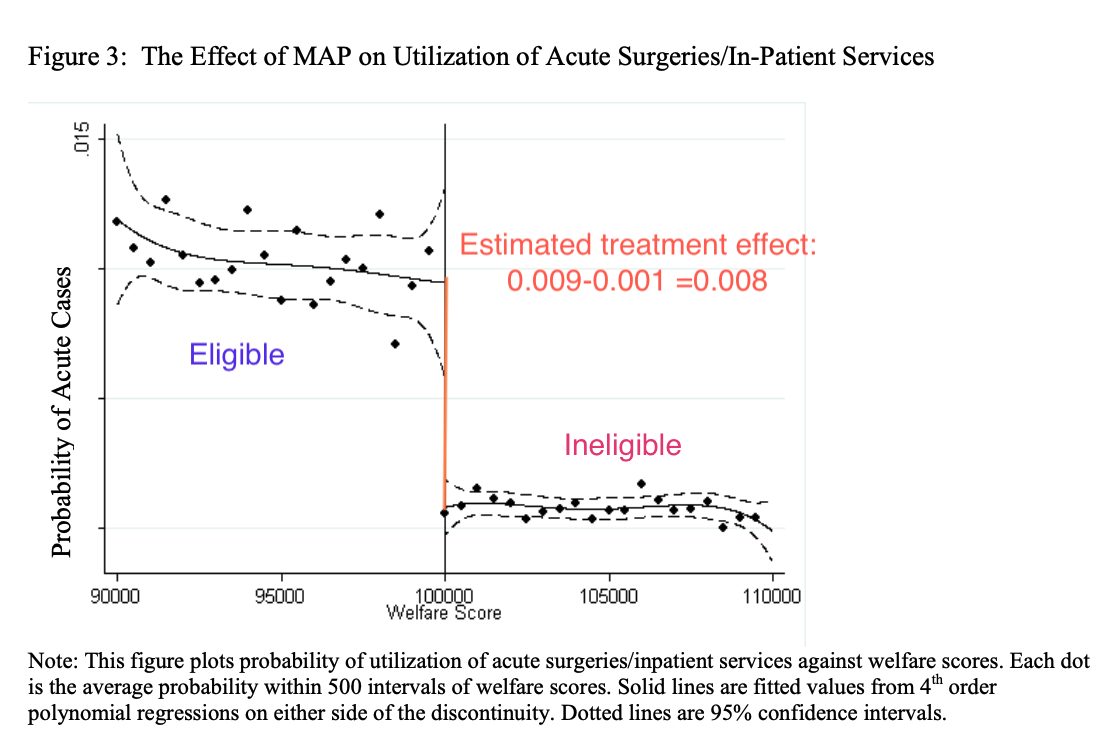
\includegraphics[width = 0.7\linewidth]{hou-rdd-treatment-effect}
	\begin{wideitemize}		
		\item
		But people just below the threshold seem to get a lot more surgeries!
		
		\item
		If everything else is continuous at the threshold, the difference is the causal effect (for people at the threshold)!
	\end{wideitemize}	
\end{frame}

\begin{frame}{Formalizing RD}
	\begin{wideitemize}
		\item
		As usual, let $D_i$ be a binary indicator for treatment (e.g. insurance status).\pause Let $R_i$ be the \textit{running variable} (e.g. the poverty score)
		
		\pause
		\item
		In a \textit{sharp} regression discontinuity design, unit $i$ receives treatment if and only if $R_i$ is above the threshold
		$$D_i = 1[ R_i \geq c ] $$
		
		(I've flipped the sign from the example to match usual convention)
		\pause\smallskip
		\begin{itemize}
		\item Note unlike before, $D_i$ is \emph{deterministic} in a likely confounder -- no room for a ``selection-on-observables'' story!
		\end{itemize}
		\item 
		The idea of RD is to compare the limits of the CEF $E[Y_i | R_i =r]$ around the cutoff $c$ (we'll assume these limits exist!):
		
		$$\tau_{RD} = \underbrace{ \lim_{r \downarrow c} E[Y_{i} | R_i = r] }_{\text{Limit from above the cutoff} }- \underbrace{\lim_{r \uparrow c} E[Y_{i} | R_i = r]}_{\text{Limit from below the cutoff} } $$
		

		\pause
		\item 
		When does $\tau_{RD}$ correspond to a causal effect? 
	\end{wideitemize}
\end{frame}

\begin{frame}{Take it to the Limit}
\begin{wideitemize}
	\item
	By definition, people with $R_i < c$ get $D_i = 0$. Thus, the limit from below the cutoff is:
	$\lim_{r \uparrow c} E[Y_{i} | R_i = r] = \pause{}  \lim_{r \uparrow c} E[Y_{i}(0) | R_i = r]$
	
	\pause
	\item 
	Similarly, people with $R_i \geq c$ get $D_i =1$. Thus, the limit from above the cutoff is
	$\lim_{r \downarrow c} E[Y_{i} | R_i = r] = \pause{} \lim_{r \downarrow c} E[Y_{i}(1) | R_i = r]$
	
	\pause
	\item
	\textbf{Key assumption:} Suppose that $f_d(r)=E[Y_{i}(d) | R_i = r]$ is \textit{continuous} at $c$ for $d= 0,1$. Then:
	\smallskip\pause{}
	\begin{itemize}
	\item $\lim_{r \uparrow c}f_0(r)=\lim_{r \uparrow c} E[Y_{i}(0) | R_i = r]=E[Y_{i}(0) | R_i = c]$\smallskip\pause{}
	\item $\lim_{r \downarrow c}f_1(r)=\lim_{r \downarrow c} E[Y_{i}(1) | R_i = r]=E[Y_{i}(1) | R_i = c]$
	\end{itemize}
	\pause
	\item
	And so
	$$\tau_{RD} =\lim_{r \downarrow c} E[Y_{i}(1) | R_i = r]- \lim_{r \uparrow c} E[Y_{i}(0) | R_i = r]\pause{} = E [Y_{i}(1) - Y_{i}(0) | R_i = c] $$
	\pause the average treatment effect for people at the cutoff!
\end{wideitemize}

\end{frame} 


\begin{frame}{Evaluating Continuity}
	\begin{wideitemize}
		\item
		The key assumption for RD is that the expectation of the potential outcomes, $E[Y_i(d) | R_i = r]$ is continuous at the cutoff (for $d=0,1$)
		
		\pause
		\item
		Why might the continuity assumption be violated?
		
		\pause
		\item
		\#1: confounding factors change discontinuously at the cutoff
		
		\pause
		\item
		\#2: people can manipulate scores to get just above/below the cutoff
		
	\end{wideitemize}
\end{frame}	

\begin{frame}{Example - Confounding Factors}
	\begin{wideitemize}
		\item
		Policies often change discontinuously at state borders
		
		\pause
		\item
		Example: Holmes (1998) is interested in how ``right-to-work laws,'' which weaken labor unions, affect businesses
		
		\pause
		\item
		He uses an RD to compare the density of manufacturing employment on both sides of borders between states that have/ \\ don't have right to work laws
	\end{wideitemize}
\end{frame}
	
	
\begin{frame}
\begin{center}
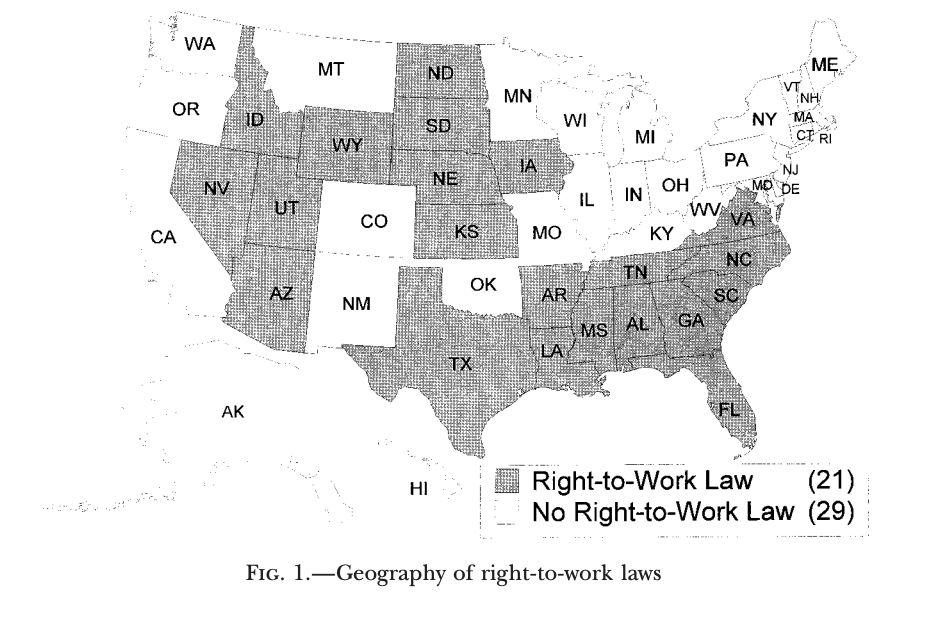
\includegraphics[width = 0.55\linewidth]{rtw-figure-2}\\
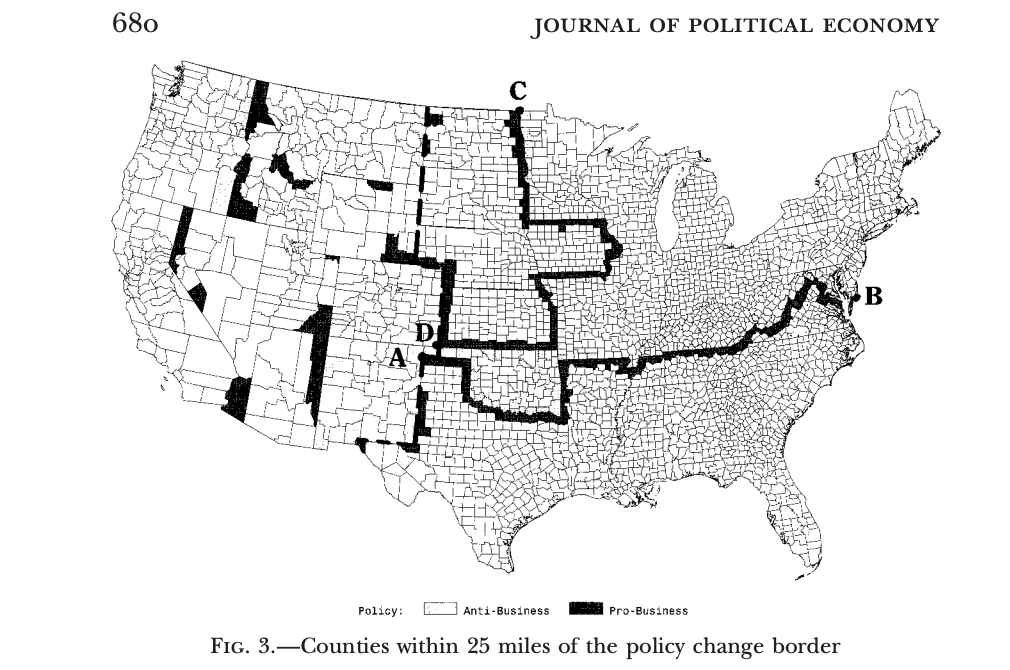
\includegraphics[width = 0.55\linewidth]{rtw-figure-1}	
\end{center}
\end{frame}	

\begin{frame}
\begin{center}
	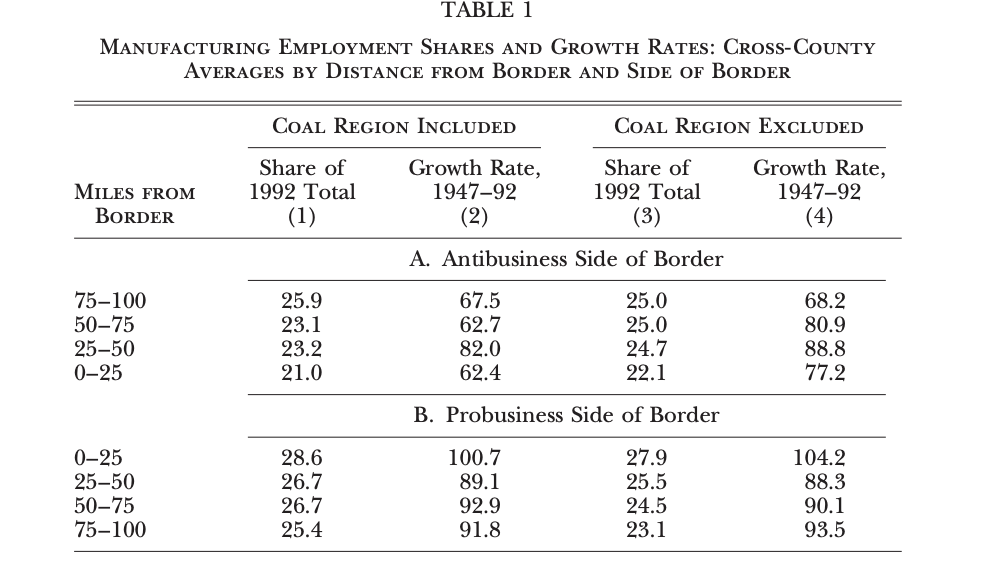
\includegraphics[width = 0.75 \linewidth]{rtw-results}
\end{center}
	\begin{wideitemize}
		\item
		There does appear to be more manufacturing just to the RTW side of state borders
		
		\pause
		\item
		But are RTWs the only thing that vary at state borders?! Could it be that RTW laws are correlated with other policies that affect manufacturing?
	\end{wideitemize}
\end{frame}

\begin{frame}
	\begin{wideitemize}
		\item
		To partially address these types of concerns, it is common to show that observable features don't vary discontinuously at the cutoff
		
		\pause
		\item
		The figure below shows that there don't appear to be any discontinuities in age, sex, education, and household size in the Hou and Chao paper
		
	\end{wideitemize}	
	\centering
	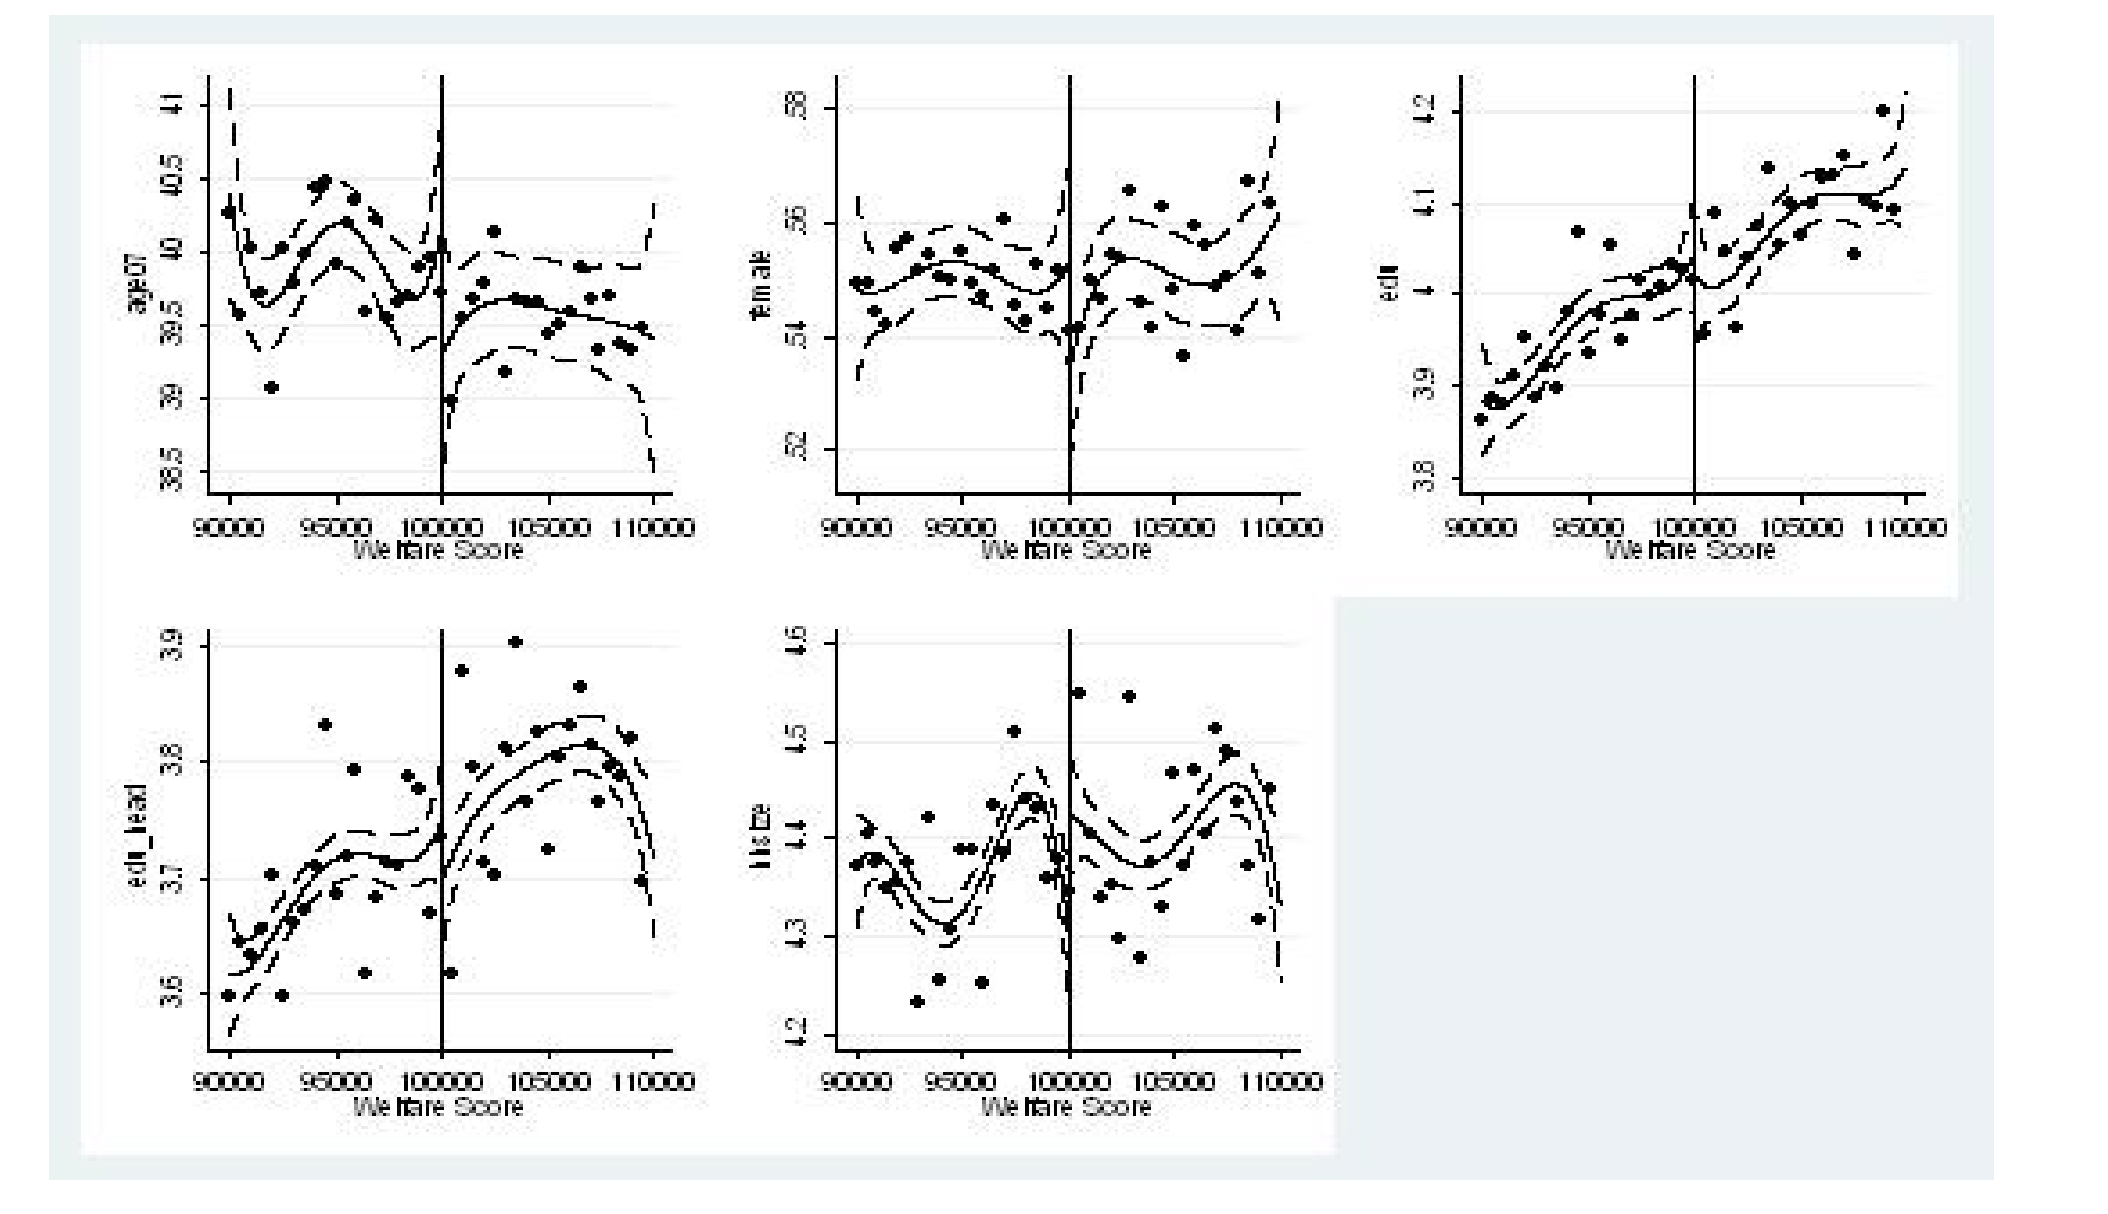
\includegraphics[width = 0.7 \linewidth]{hou-balance}

	\pause
	\begin{wideitemize}
		\item
		But as usual, there may still be concern about other unobserved confounding factors varying at the cutoff
	\end{wideitemize}
\end{frame}

\begin{frame}{Example - Manipulation}
	\begin{wideitemize}
		\item
		In NYC, students must take the Regents exams and get a score of at least 55 to get a diploma (and 65 to get a more prestigious diploma)
		
		\pause
		\item
		Might be tempted to use this to study diploma effects... But it turns out there are way more students with scores just above the thresholds
		\begin{center}
		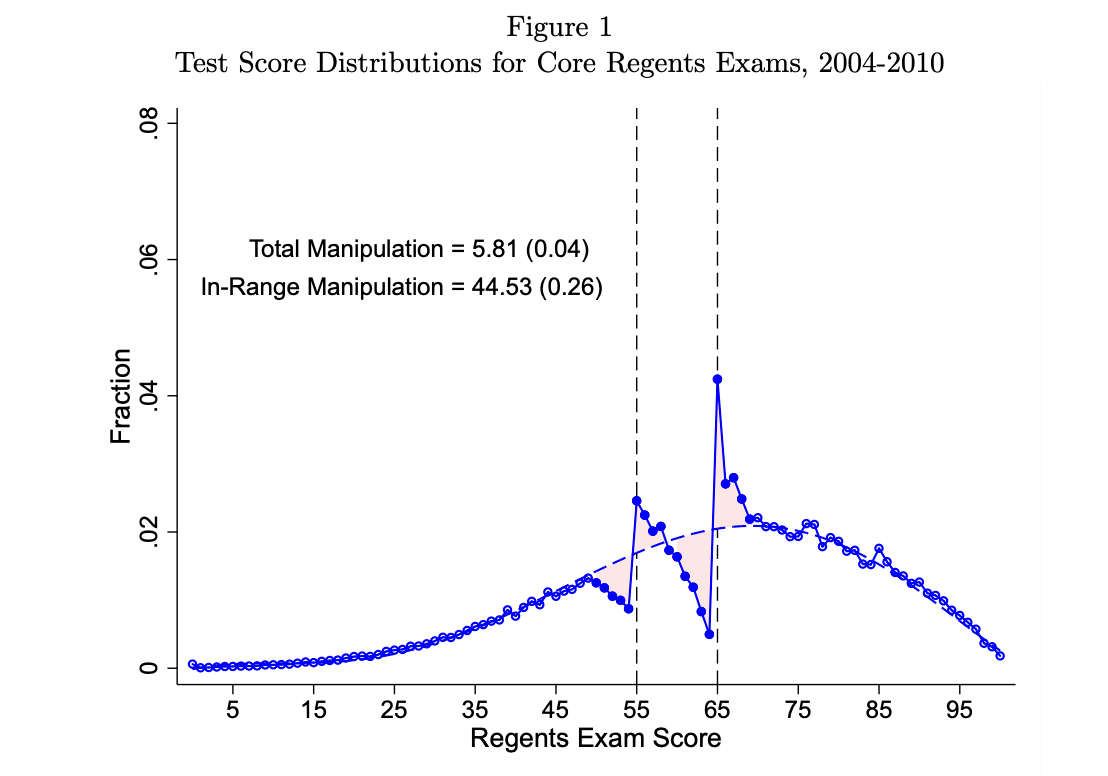
\includegraphics[width = 0.5 \linewidth]{regents-discontinuity}
		\end{center}
		
		\pause
		\item
		Likely reason: teachers cheat to bump students over the threshold
		
		\pause
		\item
		Do we think students who get bumped over the threshold versus not are similar? \pause{} Likely not, if teachers tend to bump better students...
	\end{wideitemize}
\end{frame}

\begin{frame}{Testing for Manipulation}
	\begin{wideitemize}
		\item
		To test for such RD manipulation, it is common to check whether there are a similar number of units on both sides of the cutoff. This is often called a McCrary test.
		
		\item
		If there is bunching on one side of the cutoff, this is typically interpreted as evidence of manipulation
		
		\item
		The continuity assumption will usually be much more questionable if there is bunching.
	\end{wideitemize}
\end{frame}

	
	
\begin{frame}{Estimating RD}
	\begin{itemize}
		\item 
		Under continuity, we have identification:
		$$\lim_{r \downarrow c} E[Y_{i} | R_i = r] - \lim_{r \uparrow c} E[Y_{i} | R_i = r]= E[Y_i(1)-Y_i(0)\mid R_i=c]$$ 
		
		\pause
		\item
		To estimate this CATE, all we need to do is estimate the CEF of the outcome $Y_i$ given the running variable $R_i$ and take it to the limit\bigskip
		
		\pause
		\item
		How do we estimate CEFs? \pause{} OLS!
	\end{itemize}
\end{frame}

\begin{frame}{RD with Linear Regression}
	\begin{wideitemize}
		\item
		Suppose the CEF is piecewise linear:
		\begin{align*}
			& E[Y_i | R_i = r] \approx \alpha_0 + \alpha_1 r  \hspace{2cm} \text{ if } r <c \\
			& E[Y_i | R_i = r] \approx \beta_0 + \beta_1 r \hspace{2cm} \text{ if }  r \geq c
		\end{align*}
	
	\pause
	\item
	Then under the RD assumptions, 
	$$CATE = \lim_{r \downarrow c} E[Y_{i} | R_i = r] - \lim_{r \uparrow c} E[Y_{i} | R_i = r] \approx \pause{} (\beta_0 + \beta_1 c) - (\alpha_0 + \alpha_1 c) $$
	\pause
	\item
	We can estimate these regression coefficients via OLS to estimate the effect of the treatment
	\end{wideitemize}
\end{frame}

\begin{frame}{Doing it All in One Regression}
	\begin{wideitemize}
		\item
		If we normalize $c=0$ (without loss of generality), we can actually do it all in one regression
		
		\pause
		\item
		Consider the regression:
		\begin{align*}
			Y_i  = \alpha +  \beta 1[R_i \geq 0]  + \gamma R_i  + \delta  R_i 1[R_i \geq 0 ]  + U_i
		\end{align*}
		
		\pause
		\item
		Then
		\begin{align*}
			  \text{ if } r <0, \hspace{2cm} E[Y_i | R_i = r] \approx & \pause{} \alpha + \gamma r   \\ \pause{}
			 \text{ if }  r \geq 0, \hspace{2cm} E[Y_i | R_i = r] \approx & \pause{} \alpha + \beta  + \gamma r + \delta r 
		\end{align*}
		 
		\pause
		\item
		So 
		\begin{align*}
			ATE& = \lim_{r \downarrow 0} E[Y_{i} | R_i = r] - \lim_{r \uparrow 0} E[Y_{i} | R_i = r] \\
			&\approx \pause{} (\alpha  + \beta + (\gamma + \delta) \times 0 ) - (\alpha + \gamma \times 0 ) = \pause{} \beta 
		\end{align*} 
	\end{wideitemize}
\end{frame}

\begin{frame}
\vspace{0.2cm}
	\centering
	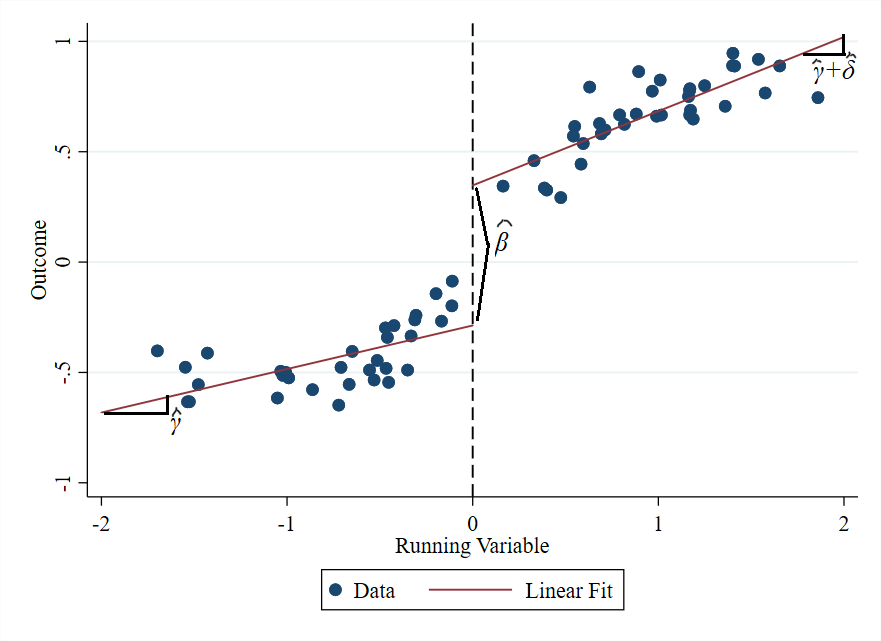
\includegraphics[width = 0.9 \linewidth]{rd_linear2}
\end{frame}


\begin{frame}{Higher Order Terms}
	\begin{wideitemize}
		\item
		This will only work well if the linear approximation to the CEF is good 
		
		\pause
		\item
		As before, we can also add higher-order terms to the regression
		
		\pause
		\item
		Here, for example, we fit a quadratic on each side:
		\begin{center}
		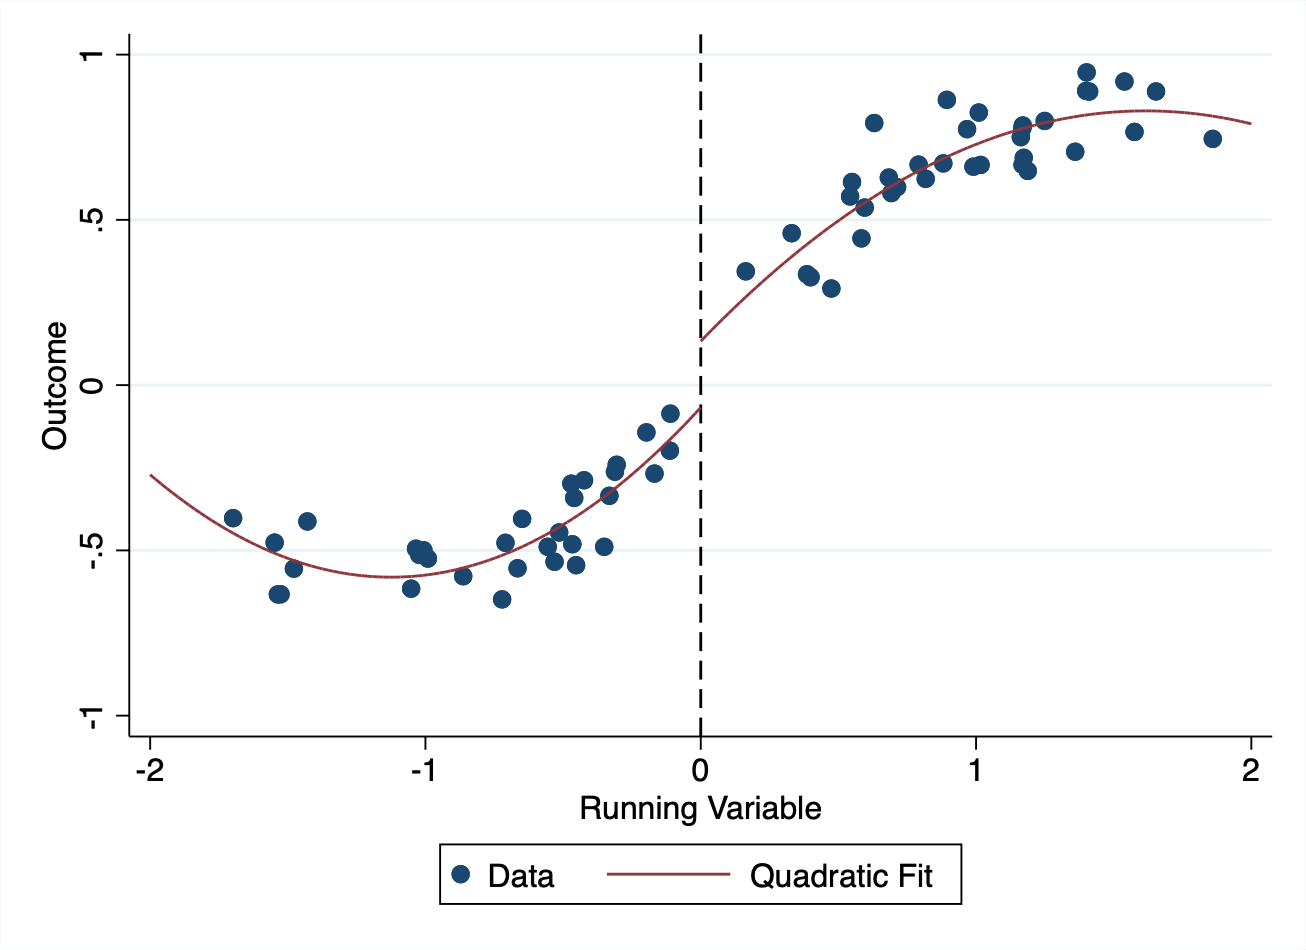
\includegraphics[width = 0.7\linewidth]{rd_quad}
		\end{center}
		
	\end{wideitemize}
\end{frame}

\begin{frame}{Problems with Higher-Order Polynomials}
	\begin{wideitemize}
		\item
		The issue with higher-order polynomials is they might overfit the data
			\begin{wideitemize}
				\item
				Particularly bad when extrapolating to the ``boundary'' of the data
			\end{wideitemize}
		
		\pause
		\item
		Is there really a discontinuity in this picture? 
		\begin{center}
		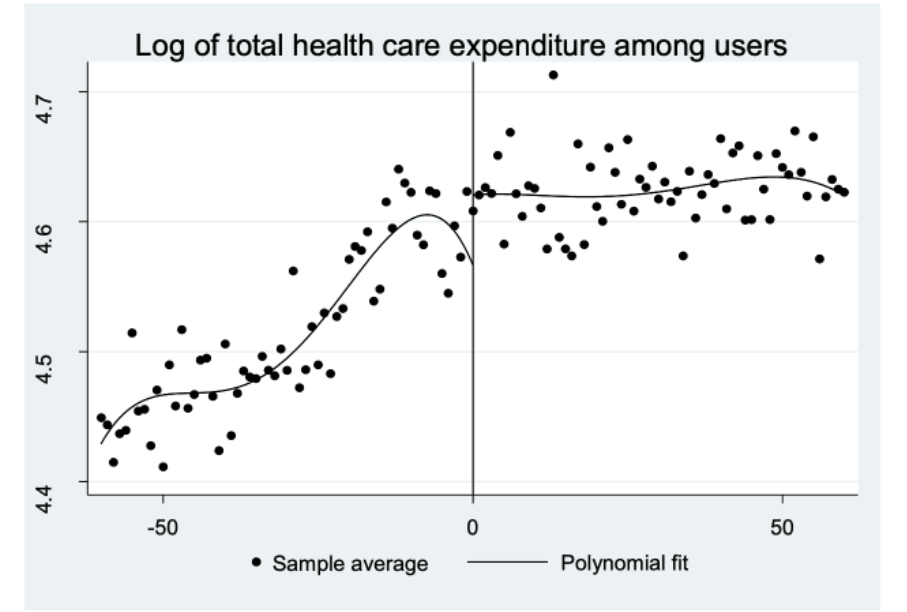
\includegraphics[width = 0.7 \linewidth]{rd-over-fitting}
		\end{center}
	\end{wideitemize}
\end{frame}

\begin{frame}{Stick to Linear?}
	The overfitting problem has led a certain Nobel laureate (and Brown graduate) to take a strong stand! \vspace{1cm}
	\begin{center}
	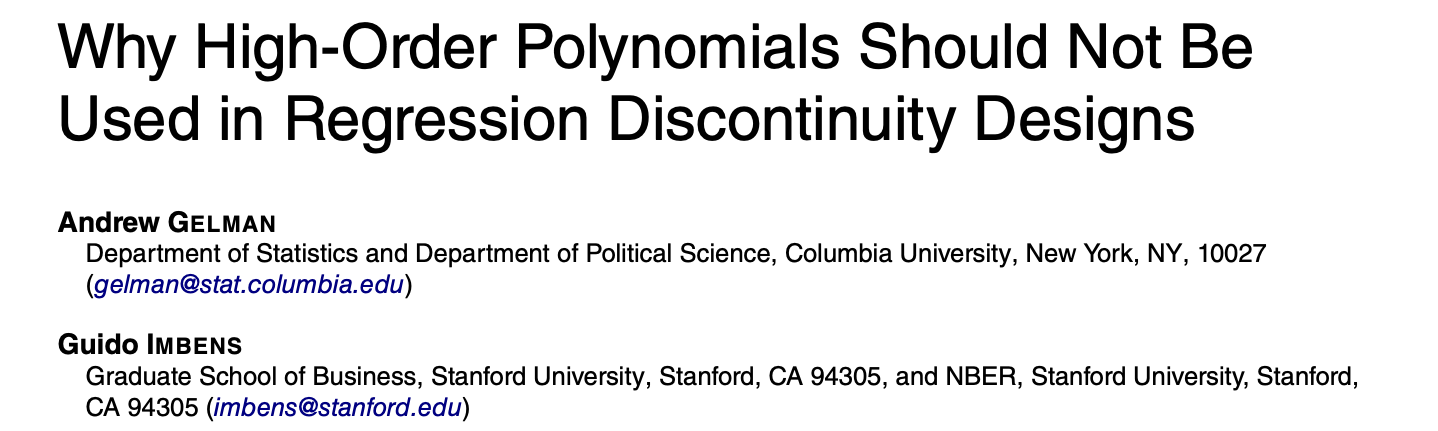
\includegraphics[width = 0.7 \linewidth]{gelman-imbens}
	\end{center}
\end{frame}

\begin{frame}{What to Do in Practice?}
	\begin{wideitemize}
		\item
		Clearly, there are tradeoffs between having a rich enough approximation to the CEF and over-fitting the data
		
		\pause
		\item
		In practice, the usual approach is to use \textbf{local linear regression}
		
		\pause
		\item
		The basic idea is to fit a linear regression but to only use points that are ``close'' to the boundary
		
				\pause
				\begin{itemize}
					\item 
					In the simplest case, just use points within a ``bandwidth'' of the cutoff
					
					\pause
					\item
					More complicated versions put higher weight on observations closer to the cutoff
				\end{itemize}
			
		\pause
		\item
		There are some data-driven ways to choose the bandwidth (e.g. use a smaller bandwidth when there are more observations)
		
		\pause
		\item
		This is easy to implement with the \texttt{rd} package in Stata	
	\end{wideitemize}
\end{frame}

\begin{frame}{Local Linear Regression}
	\begin{center}
	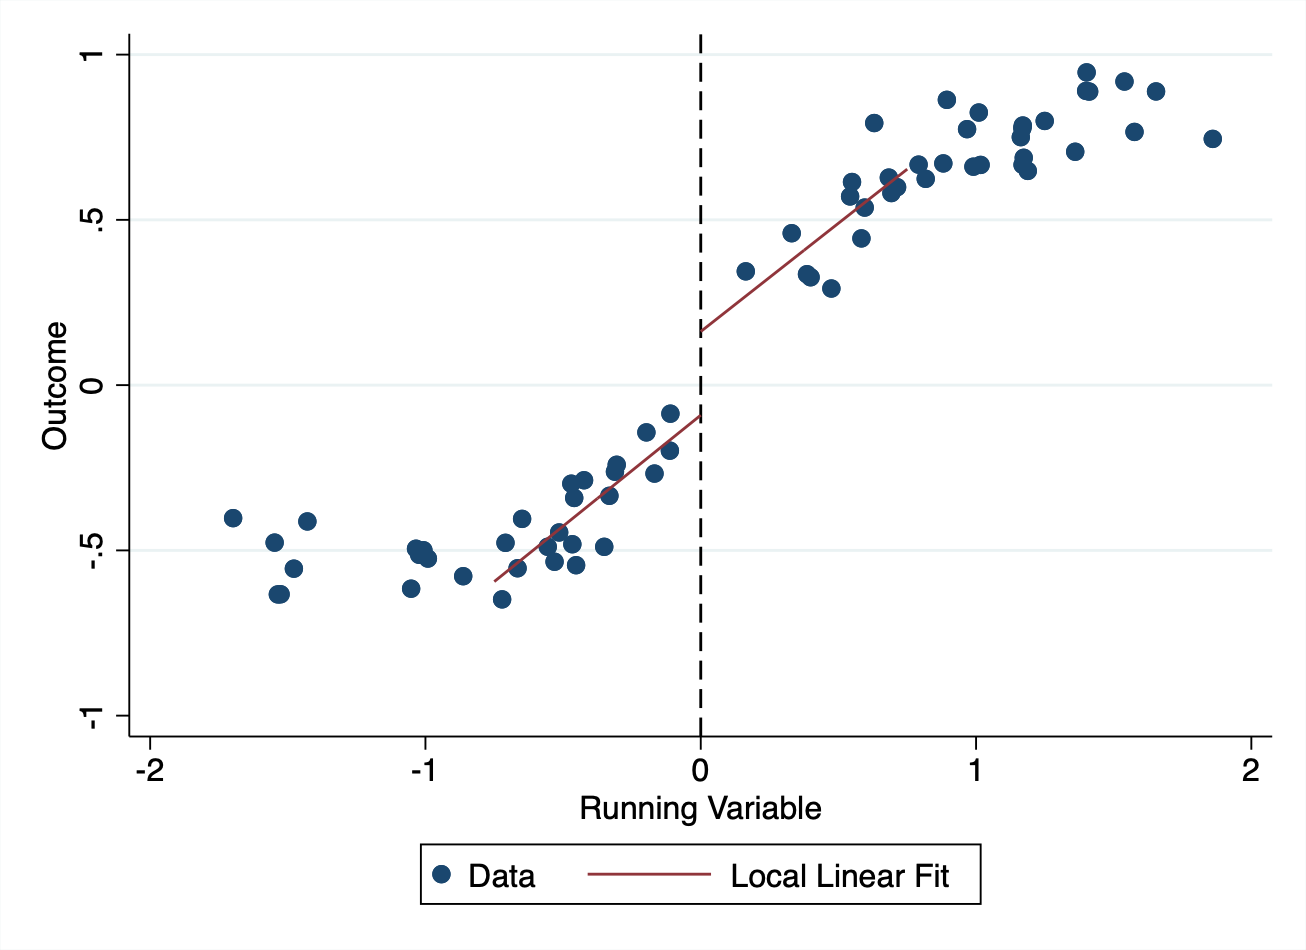
\includegraphics[width = 0.8 \linewidth]{rd_llin}
	\end{center}
\end{frame}

\begin{frame}{RD Estimation is Tricky!}
	\begin{wideitemize}
		\item
		Local linear regression is a relatively good medium between being rich enough and over-fitting
		
		\item
		But it's not perfect! In general, difficult to distinguish between a very non-linear CEF and a discontinuity
		
		\pause
		\item
		Good to trust your eyes -- does it look like there's a discontinuity on the plot?
		

		\item
		The most convincing RDs are obvious from the plot and don't need any fancy econometrics
	\end{wideitemize}
\end{frame}

%\begin{frame}{Looks Can Be Deceiving!}
%	\begin{center}
%	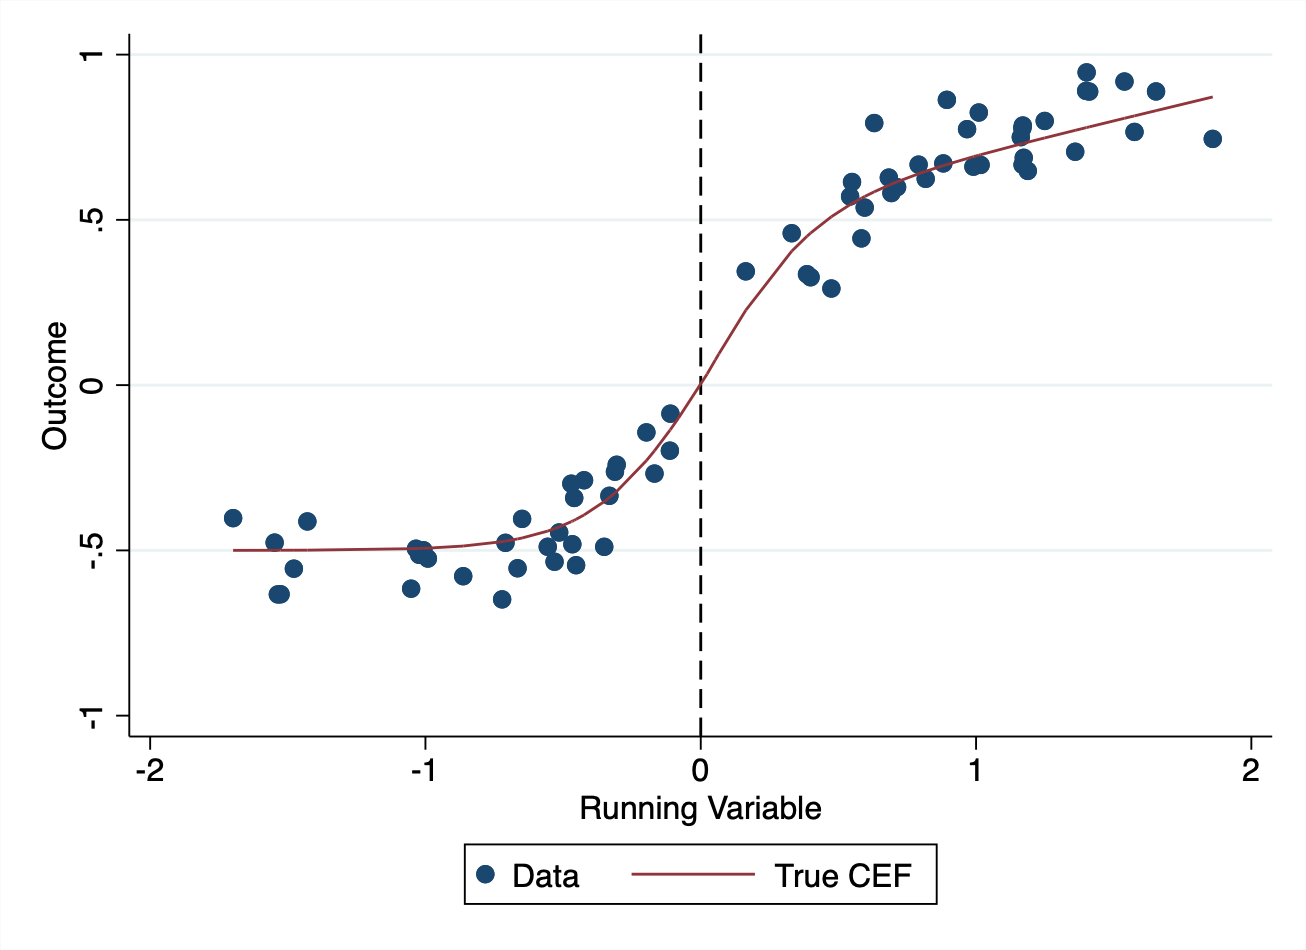
\includegraphics[width = 0.8 \linewidth]{rd_truth}
%	\end{center}
%\end{frame}

	
	
\begin{frame}{Fuzzy RD}
	\begin{wideitemize}
		\item
		Sometimes crossing a threshold doesn't completely determine treatment status, but discontinuously increases treatment probability 
		
		\item
		This is called a \textit{fuzzy} RD
		
		\pause
		\item
		The basic idea is similar to IV --- we estimate the effect of being above the threshold on the outcome, then divide this by the effect on the treatment (i.e. the change treatment probability)
		
		\pause
		\item
		Under certain conditions, this will identify the LATE at the cutoff
	\end{wideitemize}
\end{frame}

\begin{frame}{Example -- Bleemer and Mehta (2022)}
	\begin{wideitemize}
		\item
		Bleemer and Mehta ask a very important question (for you): does majoring in economics make you rich?
		
		\pause
		\item
		They study this Q in the context of UC Santa Cruz (UCSC), where the econ department only allowed people with GPA below 2.8 in intro classes to major in econ ``at the discretion of the department''
	\end{wideitemize}
\end{frame}

\begin{frame}{First Stage}
	\centering
	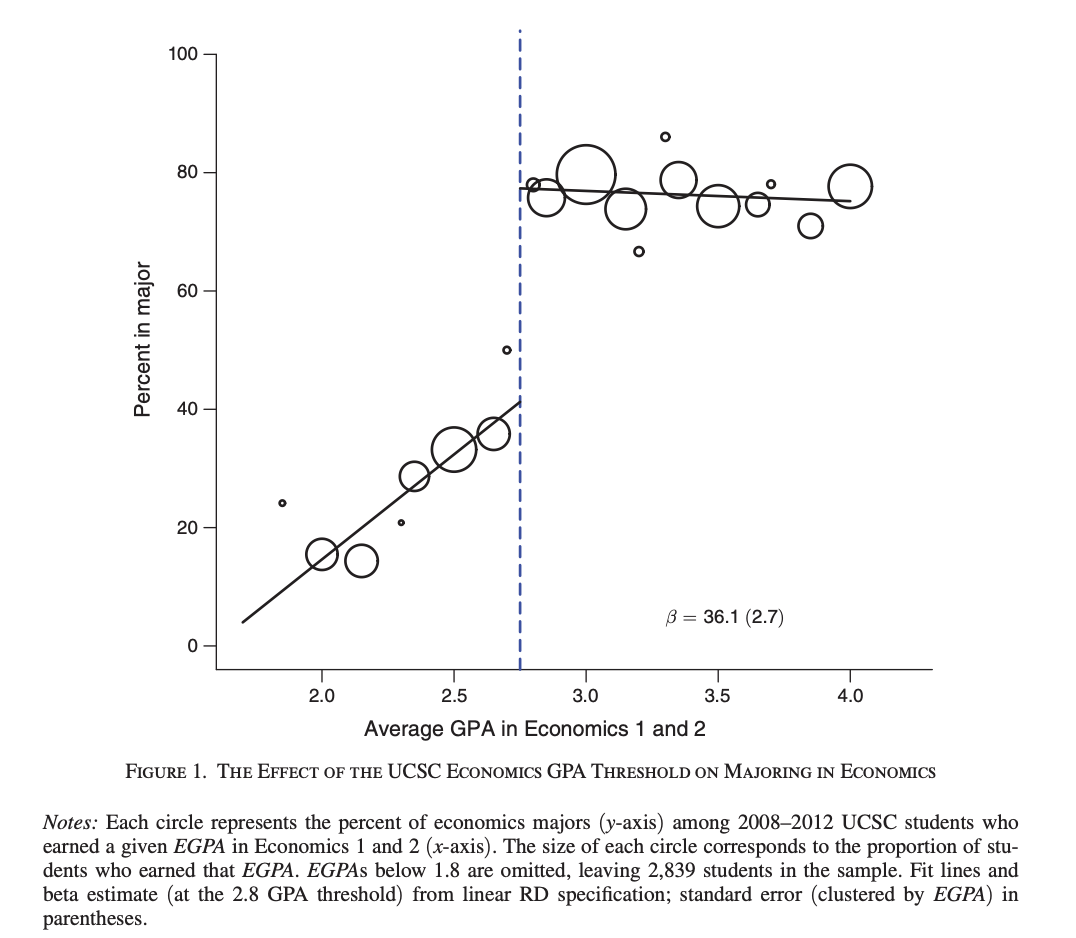
\includegraphics[width = 0.7 \linewidth]{bleemer-first-stage}
	
	Students above the threshold about 36 pp more likely to major in econ
\end{frame}

\begin{frame}
	\centering
	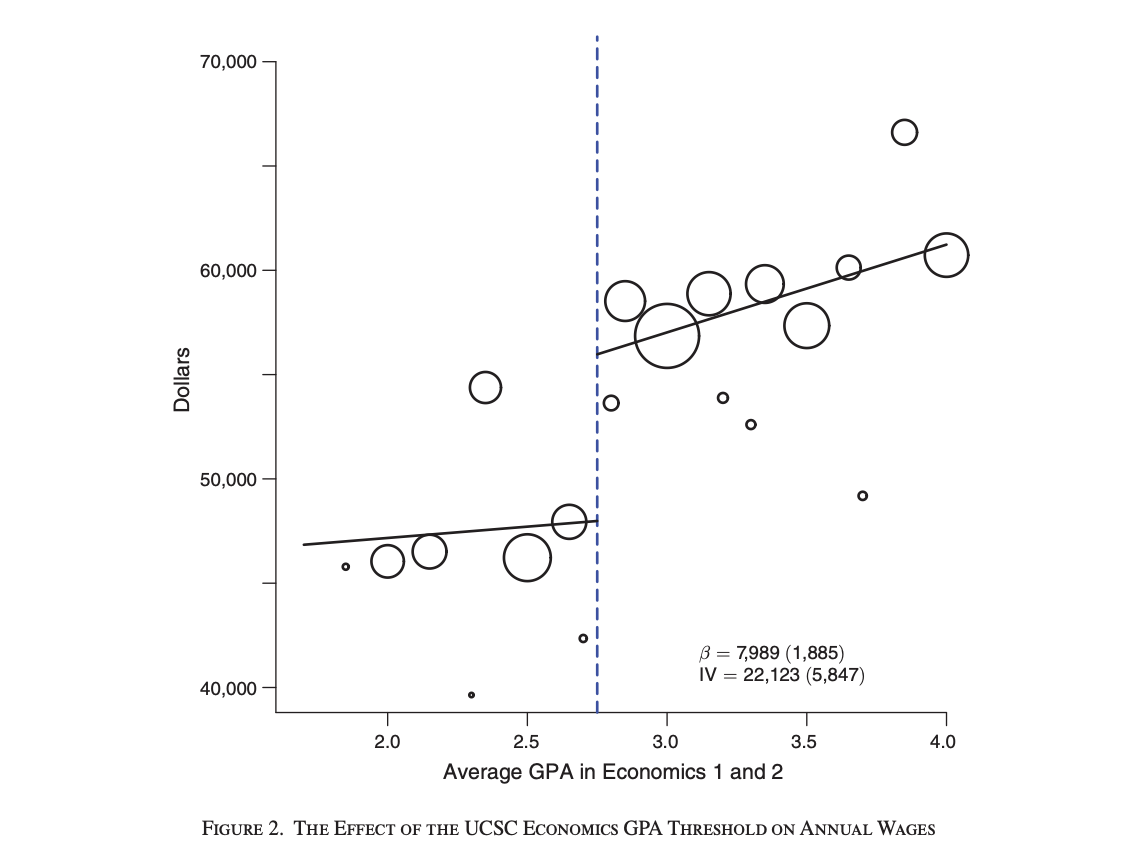
\includegraphics[width= 0.7 \linewidth]{bleemer-rf}
	
	\begin{wideitemize}
		\item
		Students about the threshold earn about \$8K more
		
		\pause
		\item
		Aren't you glad you took this course?!
		
		\pause
		\item
		The fuzzy RD estimate of the effect of majoring in econ is then $\$8K / 0.36 \approx 22K$, or 40\% of mean earnings 
	\end{wideitemize}
\end{frame}	

\begin{frame}{When does Fuzzy RD Give a LATE?}
	\begin{wideitemize}
		\item
		Under similar assumptions to those for IV, fuzzy RD gives a LATE for compliers at the cutoff
		
		\pause
		\item
		\textbf{Continuity}. Need that $E[Y_i(d) | R_i]$ is continuous at the cutoff for $d=0,1$
		
		
		\item
		\textbf{Exclusion}. Being just above/below the cutoff affects outcomes only through its effect on treatment
		
		
		\item \textbf{Relevance}. There is a discontinuity in treatment takeup at the cutoff. 
		
		
		\item \textbf{``Local'' Monotonicity}. No defiers who only take treatment if below the cutoff.
	\end{wideitemize}
\end{frame}


\begin{frame}{Dell and Querubin (2017)}
\begin{wideitemize}
	\item
	Dell and Querubin exploit the fact that during the Vietnam War, the US airforce selected bombing targets based on a risk score formed using 169 security/political/economic characteristics of villages
	
	\item
	The algorithm produced a continuous score which was rounded to the nearest integer before being given to generals $\rightarrow$ Dell and Querubin exploit the discontinuity from rounding
\end{wideitemize}	
\centering 
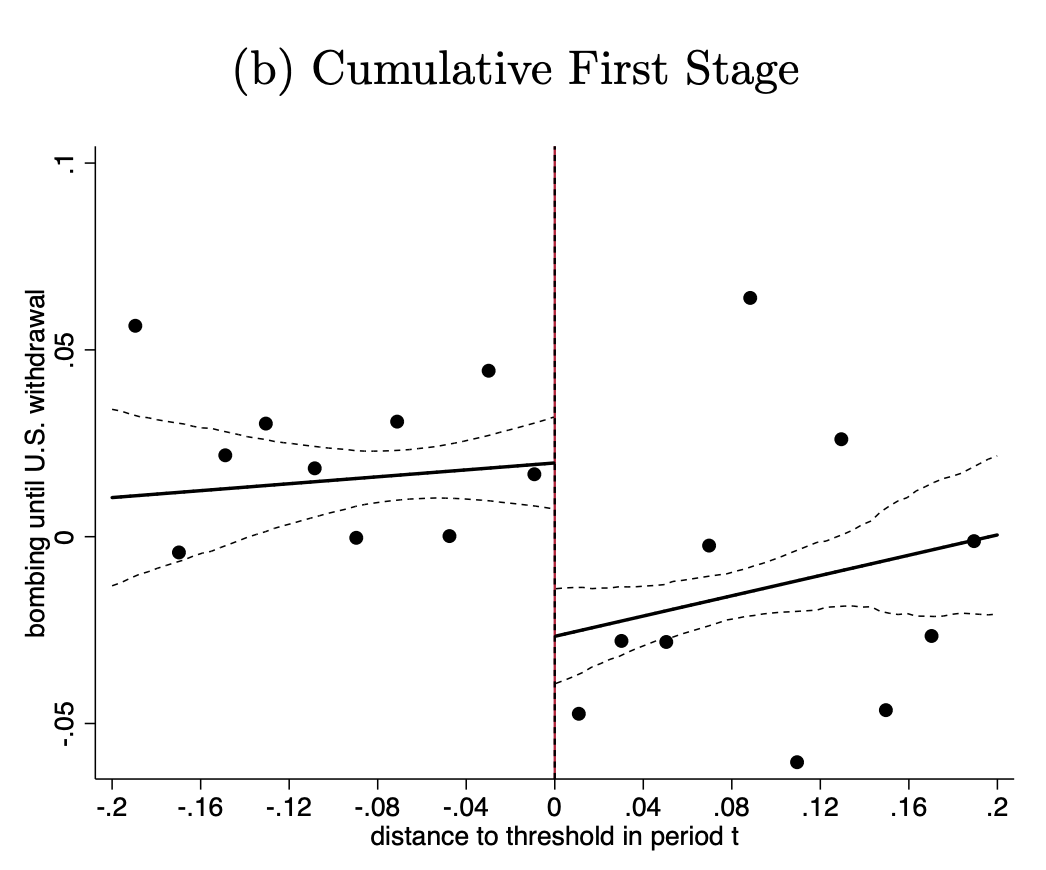
\includegraphics[width = 0.5\linewidth]{dell-first-stage}
\end{frame}

\begin{frame}{Checking for Balance}
	\begin{wideitemize}
		\item
		Areas above/below the threshold have similar characteristics prior to bombing decision
		
		\item
		E.g., they have similar \# of bombings prior to when score was used
	\end{wideitemize}

\centering 
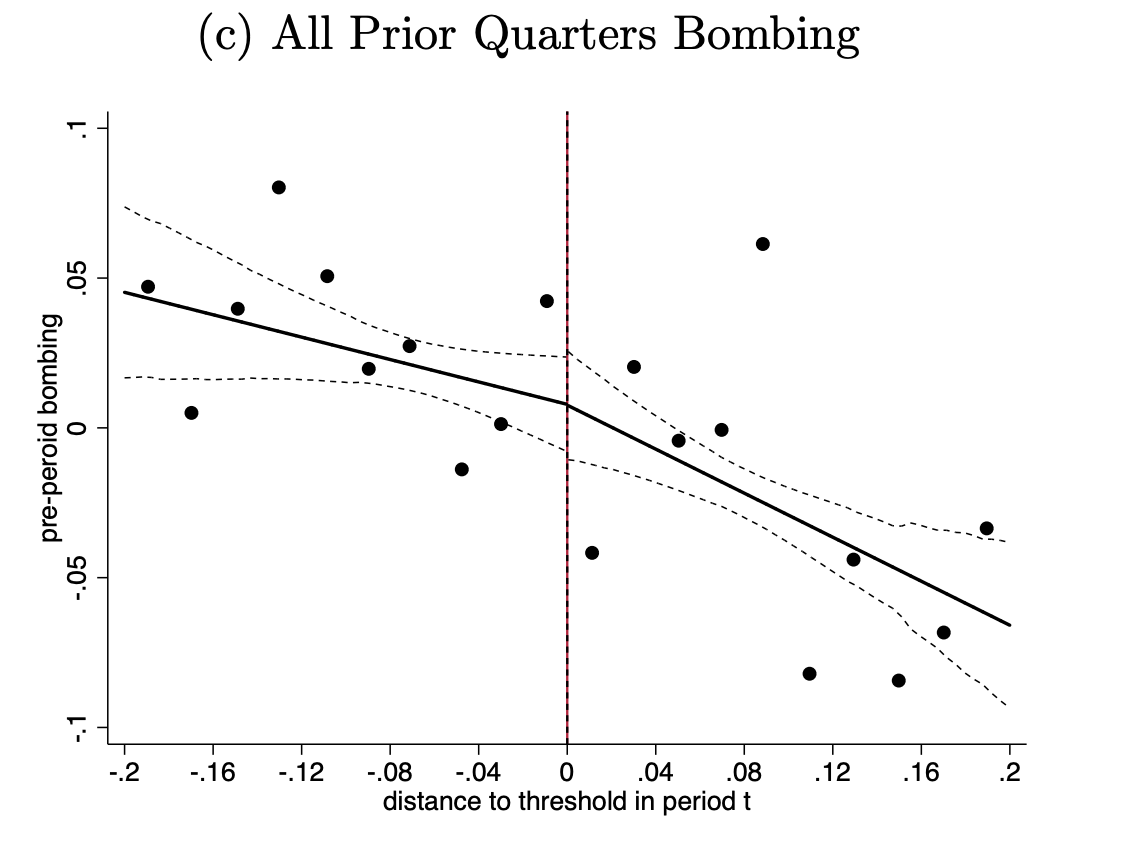
\includegraphics[width = 0.7\linewidth]{dell-balance}
\end{frame}

\begin{frame}

\begin{wideitemize}
	\item
	Bombing appears to be bad for villages $\rightarrow$ fewer schools
\end{wideitemize}

\centering 
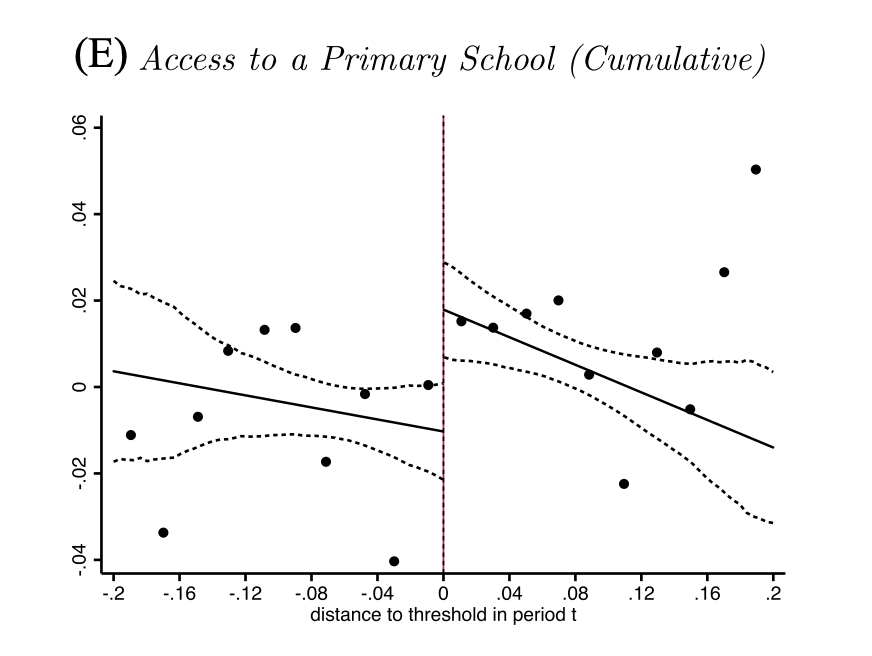
\includegraphics[width = 0.7\linewidth]{dell-schools}	
\end{frame}

\begin{frame}
	
	\begin{wideitemize}
		\item
		Bombing also appears to be bad for military objectives $\rightarrow$ more long-run Vietcong (VC) activity
	\end{wideitemize}
	
	\centering 
	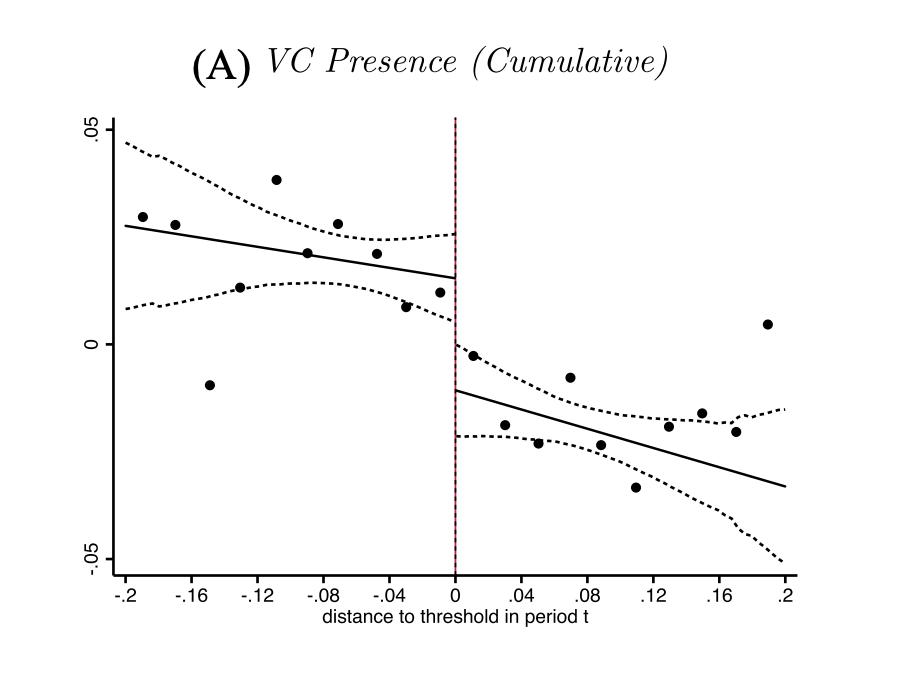
\includegraphics[width = 0.7\linewidth]{dell-vc}	
\end{frame}

\begin{frame}{So to Conclude...}
	\begin{wideitemize}
		\item
		Bombing is bad $\checkmark$
		
		\item
		Econometrics is good $\checkmark$
		
	\end{wideitemize}
\end{frame}


\end{document}


